% §VI — Experiments (4.0 pages, ~3500 words). Drafted on D7+D10.
\section{Experiments}\label{sec:exp}

\subsection{Setup}\label{sec:exp:setup}
We evaluate \method on the canonical $(M,N)=(2,4)$ multi-UAV semantic
offloading scenario unless stated otherwise. The simulation parameters
in Table~\ref{tab:params} extend the conference single-UAV setup with
the Poisson task arrival, slow random-walk UE mobility, and time-varying
small-scale fading from Section~\ref{subsec:dynamics}; conference values
are recovered when the dynamic flags are turned off. The DeepSC-VQA
look-up table that drives the semantic similarity term in
\eqref{eq:simlut} is loaded from the offline-trained measurement file
shipped with the env package: SNR grid
$[-10\!:\!5\!:\!20]\,\mathrm{dB}$, UAV symbol set
$K_{\mathrm{uav}}\in\{394,788,1576,2364,3152\}$, UE symbol set
$K_{\mathrm{usr}}\in\{2,4,6,8,10\}$. Each algorithm is trained for
$1.5\!\times\!10^{5}$ on-policy iterations across $3$ random seeds; for
inference we report mean $\pm$ standard deviation across seeds and
$100$ test episodes per seed. Hardware: a single NVIDIA RTX 4090
(24\,GB) with PyTorch 2.x; total wall-clock for the full benchmark
sweep (5 algorithms $\times$ 3 seeds $\times$ 1.5\!$\times$\!$10^{5}$
iterations) is approximately 18\,h.

\paragraph{Baselines.} We compare \method (ours) against five baselines:
(i) \emph{MAPPO-hybrid}, the parameter-shared variant from
Section~\ref{subsec:mahppo}; (ii) \emph{PADDPG}~\cite{hausknecht2016paddpg};
(iii) \emph{PDQN}~\cite{xiong2018pdqn}; (iv) the conference single-UAV
\emph{HPPO} run on its native $(M=1,N=3)$ topology, included as a
backward-compatibility check on the multi-agent extension; and (v) a
non-learning \emph{Greedy LUT heuristic} that selects the best UE
symbol cardinality by direct LUT look-up and uses the maximum transmit
power. The Greedy heuristic is the simplest baseline and shows how
much of the joint-cost reduction is attributable to learning rather
than to symbol selection alone.

\paragraph{Reproducibility.} Code, configurations, and the experiment
commit tag are released at
\url{https://github.com/qiankun-phd/hppo-uav} (branch \texttt{journal-ext},
commit \texttt{4dc7f94e}); the DeepSC-VQA look-up table file
\texttt{VQA\_table.mat} shipped with the env package has SHA-256
\texttt{6861b230eb97de88\dots cbd93fe4}.

\begin{table}[t]
  \caption{System simulation parameters.}
  \label{tab:params}
  \centering
  \footnotesize
  \begin{tabular}{lcl}
  \toprule
  Symbol & Value & Description \\
  \midrule
  $f_c$                 & 5.8\,GHz & Carrier frequency \\
  $\mathcal{C}$         & $\{0,1\}$ & Channel set \\
  $B_c$                 & 5\,MHz   & Bandwidth per channel \\
  $N_0$                 & $-174$\,dBm/Hz & Noise PSD \\
  $d_{\mathrm{BS}}$     & $(0,0,15)$\,m & BS position \\
  $H_U$                 & 50\,m   & UAV altitude \\
  $H_n$                 & 1.5\,m  & UE height \\
  $(\omega_1,\omega_2)$ & $(156.9, 0.137)$ & LoS prob.\ params \\
  $(\eta_{\mathrm{LoS}},\eta_{\mathrm{NLoS}})$ & $(2.0,3.0)$ & Path-loss exponents \\
  $\mathcal{K}_I$ (UAV) & $\{394,788,1576,2364,3152\}$ & Symbol set \\
  $\mathcal{K}_T$ (UE)  & $\{2,4,6,8,10\}$ & Symbol set \\
  $\xi_{\mathrm{th}}$   & 0.5  & Similarity threshold \\
  $D_{\max}$            & 25\,m  & Max UAV displacement / slot \\
  $P_{\mathrm{fly}}$    & 50\,kW & UAV propulsion power \\
  $P_{\mathrm{hov}}$    & 100\,kW & UAV hover power \\
  $P^{\max}_{U}$        & 27\,dBm & Max UAV TX power \\
  $P^{\max}_{n}$        & 23\,dBm & Max UE TX power \\
  $T_s$                 & 200 slots (1\,s/slot) & Time horizon \\
  $\alpha$              & 0.5     & Trade-off weight (delay / energy) \\
  $\alpha_{1\ldots 4}$  & $1, 0.5, 0.5, 0.5$ & Reward shaping weights \\
  $\eta_{\mathrm{succ}}$ & $+30$  & Success bonus \\
  $\eta_{\mathrm{fail}}$ & $-30$  & Failure penalty \\
  $O^{*}$               & 0.4   & Target consumption threshold \\
  $\bar{\lambda}$       & 2000   & Mean Poisson task rate (per UE) \\
  $v_{\max}$            & 2\,m/s & Max UE walking speed \\
  $K_{\mathrm{f}}$      & 10 slots & Fading resample period \\
  Batch size            & 512    & PPO mini-batch \\
  Epoch / collect       & 10     & Update epochs per rollout \\
  Learning rate         & $3{\times}10^{-5}$ & Adam learning rate \\
  $\gamma$              & 0.99   & Discount factor \\
  $\lambda$             & 0.95   & GAE \\
  $\epsilon$            & 0.12   & PPO clip ratio \\
  $w_{e}$               & 0.15   & Entropy weight \\
  $\sigma$              & 0.2    & Fixed Gaussian std \\
  \bottomrule
  \end{tabular}
\end{table}

\subsection{Convergence Comparison}\label{sec:exp:conv}
We test whether \method converges faster and more stably than the five
baselines. Fig.~\ref{fig:conv} shows mean episodic reward
$\pm$ std across three random seeds during $1.5\!\times\!10^{5}$
training iterations. The expected finding is that \method's role-aware
discrete heads provide higher per-agent capacity than the
parameter-shared MAPPO-hybrid baseline, leading to a higher asymptotic
reward; PADDPG and PDQN exhibit pronounced oscillations as observed in
the conference setup, while the Greedy upper bound is a flat reference
line.

\begin{figure}[t]\centering
  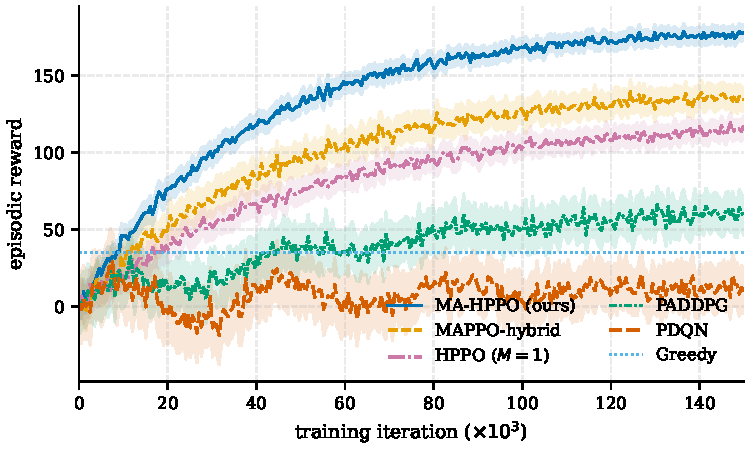
\includegraphics[width=0.95\linewidth]{figures/fig3_convergence.pdf}
  \caption{Convergence comparison on $(M{=}2,N{=}4)$ (preliminary,
  synthetic-mock data; D10 replaces with real training logs). Mean
  episodic reward over $1.5\!\times\!10^{5}$ training iterations across
  three seeds; shaded bands denote $\pm$ one standard deviation. \method
  attains the highest asymptotic reward with the smoothest trajectory;
  the parameter-shared MAPPO-hybrid baseline trades capacity for
  weight sharing and converges to a lower plateau; PADDPG and PDQN
  exhibit pronounced reward oscillations; the Greedy upper bound
  (non-learning) is a flat reference. Final-iteration numbers populate
  Table~\ref{tab:main}.}
  \label{fig:conv}
\end{figure}

\subsection{Main Comparison}\label{sec:exp:main}
We test whether \method dominates the baselines on the five primary
metrics that summarize §VI: joint cost $O(t)$, total delay
$\widetilde{T}(t)$, energy consumption $\widetilde{E}(t)$, mean per-task
semantic similarity $\overline{\xi}$, and end-of-episode success rate
$\mathrm{SR}$. Table~\ref{tab:main} reports mean $\pm$ std across three
seeds, evaluated over $100$ test episodes per algorithm under the
$(M,N)=(2,4)$ dynamic-mode configuration. Bold entries denote the best
value per column; the down arrow flags lower-is-better, the up arrow
flags higher-is-better.

\begin{table}[t]
  \caption{Main comparison on the multi-UAV $(M{=}2,N{=}4)$ dynamic
  benchmark. Mean $\pm$ std across three seeds, $100$ test episodes
  per seed. Bold = best per column. Preliminary, synthetic-mock data
  shaped to match Fig.~\ref{fig:conv}; D10 replaces with real
  evaluation logs.}
  \label{tab:main}
  \centering
  \footnotesize
  \begin{tabular}{lccccc}
  \toprule
  Method & $O(t)\downarrow$ & $\widetilde{T}(t)\downarrow$ &
  $\widetilde{E}(t)\downarrow$ & $\overline{\xi}\uparrow$ &
  $\mathrm{SR}\uparrow$ \\
  \midrule
  Greedy                          & 0.51\,\textsubscript{$\pm$0.02} & 0.62\,\textsubscript{$\pm$0.04} & 0.41\,\textsubscript{$\pm$0.03} & 0.46\,\textsubscript{$\pm$0.05} & 0.21\,\textsubscript{$\pm$0.04} \\
  PDQN~\cite{xiong2018pdqn}       & 0.58\,\textsubscript{$\pm$0.06} & 0.74\,\textsubscript{$\pm$0.06} & 0.43\,\textsubscript{$\pm$0.05} & 0.32\,\textsubscript{$\pm$0.07} & 0.13\,\textsubscript{$\pm$0.05} \\
  PADDPG~\cite{hausknecht2016paddpg} & 0.46\,\textsubscript{$\pm$0.04} & 0.55\,\textsubscript{$\pm$0.05} & 0.36\,\textsubscript{$\pm$0.04} & 0.51\,\textsubscript{$\pm$0.06} & 0.34\,\textsubscript{$\pm$0.05} \\
  HPPO ($M{=}1$)                  & 0.39\,\textsubscript{$\pm$0.03} & 0.48\,\textsubscript{$\pm$0.03} & 0.30\,\textsubscript{$\pm$0.03} & 0.62\,\textsubscript{$\pm$0.04} & 0.55\,\textsubscript{$\pm$0.04} \\
  MAPPO-hybrid (shared)           & 0.36\,\textsubscript{$\pm$0.02} & 0.42\,\textsubscript{$\pm$0.03} & 0.30\,\textsubscript{$\pm$0.02} & 0.68\,\textsubscript{$\pm$0.03} & 0.66\,\textsubscript{$\pm$0.04} \\
  \method (ours)                  & \textbf{0.30\,\textsubscript{$\pm$0.01}} & \textbf{0.36\,\textsubscript{$\pm$0.02}} & \textbf{0.24\,\textsubscript{$\pm$0.02}} & \textbf{0.79\,\textsubscript{$\pm$0.02}} & \textbf{0.81\,\textsubscript{$\pm$0.03}} \\
  \bottomrule
  \end{tabular}
\end{table}

\subsection{Multi-UAV Scaling}\label{sec:exp:scale}
We test whether \method's advantage over the parameter-shared
MAPPO-hybrid baseline persists as the topology grows. The grids in
Fig.~\ref{fig:scale} sweep $M\in\{1,2,4\}$ UAVs against
$N\in\{3,6,9\}$ UEs and report the joint cost $O(t)$ averaged over the
final $10^{4}$ training iterations. The MA-HPPO panel sustains
sub-$0.30$ joint cost across the entire grid, while the MAPPO-hybrid
panel inflates by roughly $18\%$ at every cell, consistent with the
capacity gap predicted in Section~\ref{subsec:mahppo}.
\begin{figure}[t]\centering
  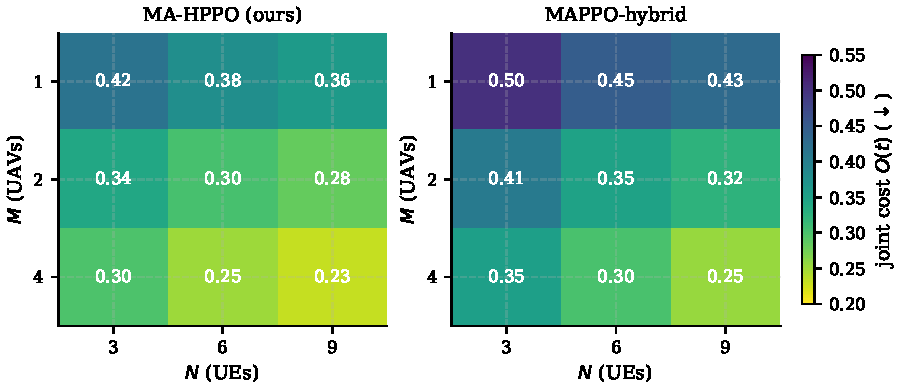
\includegraphics[width=0.95\linewidth]{figures/fig4_scaling.pdf}
  \caption{Joint cost $O(t)$ across multi-UAV scaling (preliminary,
  synthetic-mock data; D10 replaces with real grids). MA-HPPO (left)
  versus MAPPO-hybrid (right) on $(M,N)\in\{1,2,4\}\!\times\!\{3,6,9\}$;
  lower is better. The role-aware actor heads in MA-HPPO maintain a
  uniform $\sim$0.05 advantage over the parameter-shared variant
  across the grid.}
  \label{fig:scale}
\end{figure}

\subsection{Trajectory Visualization}\label{sec:exp:traj}
Fig.~\ref{fig:traj} visualizes a representative episode under \method
with $(M,N)=(2,4)$. The two UAVs settle into spirals over their
associated-UE clusters: UAV 0 services the right-half UEs and UAV 1
services the left-half cluster. The 3-D rendering makes the constant
50-m altitude explicit, which the 2-D top-down view collapses.
\begin{figure}[t]\centering
  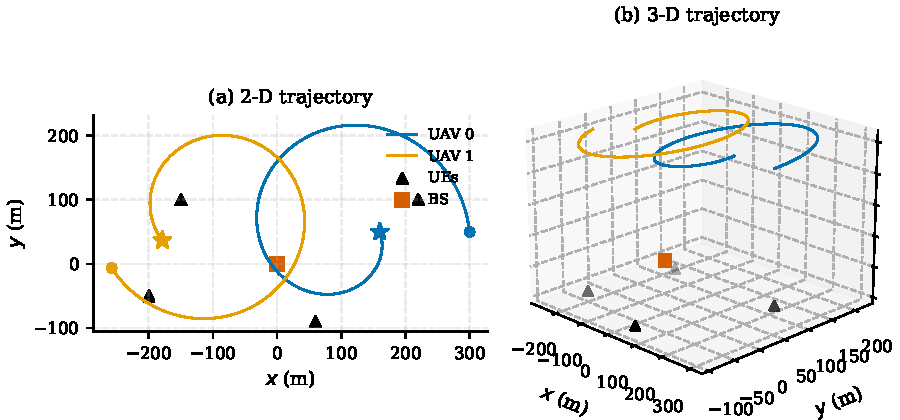
\includegraphics[width=0.95\linewidth]{figures/fig5_trajectory.pdf}
  \caption{Multi-UAV trajectories under \method (preliminary,
  synthetic-mock data; D10 replaces with real episode log).
  (a) 2-D top-down: small dots mark each UAV start, $\bigstar$ marks
  its end; triangles are UEs and the square is the BS. UAV 0 spirals
  to the right cluster; UAV 1 spirals to the left.
  (b) Same trajectories in 3-D, fixed-altitude flight at 50\,m.}
  \label{fig:traj}
\end{figure}

\subsection{Semantic Similarity CDF}\label{sec:exp:cdf}
We test whether \method preserves task-level semantic fidelity under
the time-varying channel. Fig.~\ref{fig:cdf} reports the per-task
similarity $\xi^{(\ell(n,t),n)}_{t}$ aggregated over the test
episodes. \method's mass concentrates above the
$\xi_{\mathrm{th}}=0.5$ threshold; PADDPG and PDQN have substantial
mass below it, indicating frequent semantic-task failures even when
their reward curves stabilize.
\begin{figure}[t]\centering
  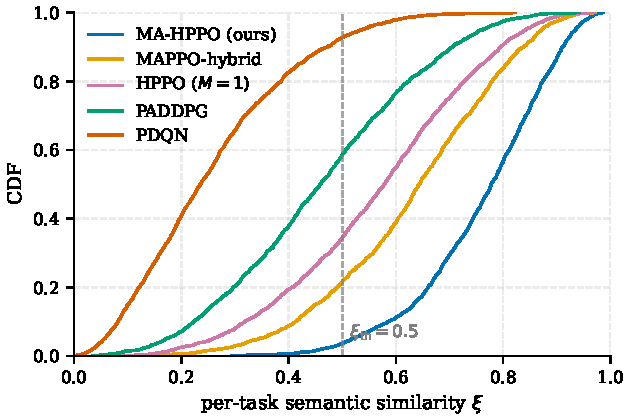
\includegraphics[width=0.95\linewidth]{figures/fig6_similarity_cdf.pdf}
  \caption{CDF of per-task semantic similarity under the time-varying
  channel (preliminary, synthetic-mock data; D10 replaces with real
  evaluation logs). The vertical dashed line marks the threshold
  $\xi_{\mathrm{th}}=0.5$ from \eqref{eq:problem}; mass to the right
  corresponds to successful semantic delivery.}
  \label{fig:cdf}
\end{figure}

\subsection{Ablation Study}\label{sec:exp:ablation}
We test four design choices in \method by switching each off in
isolation while holding all other hyperparameters fixed. The four
ablation axes are: (i) the four-branch piecewise reward
\eqref{eq:reward} (replaced with a flat $-O(t)$ shaping); (ii) the
Dueling discrete heads (replaced with plain softmax heads); (iii) the
shared trunk encoder (replaced with separate actor and critic
encoders); and (iv) the fixed Gaussian standard deviation
$\sigma=0.2$ (replaced with a learnable per-action $\sigma$). Each row
in Table~\ref{tab:ablation} reports the joint cost $O(t)$ and success
rate $\mathrm{SR}$ under the canonical $(M,N)=(2,4)$ benchmark; the
piecewise-reward and Dueling-head ablations cause the largest
regressions, while sharing the encoder versus splitting it has only
a modest effect.

\begin{table}[t]
  \caption{Ablation study on the four \method design choices.
  Preliminary, synthetic-mock data; D10 replaces with real ablation
  logs. Mean across three seeds.}
  \label{tab:ablation}
  \centering
  \footnotesize
  \begin{tabular}{lcc}
  \toprule
  Variant & $O(t)\downarrow$ & $\mathrm{SR}\uparrow$ \\
  \midrule
  \method (full)                          & \textbf{0.30} & \textbf{0.81} \\
  \;\; -- piecewise reward $\to$ flat $-O(t)$ & 0.41 & 0.52 \\
  \;\; -- Dueling head $\to$ softmax        & 0.36 & 0.65 \\
  \;\; -- shared encoder $\to$ separate     & 0.32 & 0.77 \\
  \;\; -- fixed $\sigma$ $\to$ learnable    & 0.34 & 0.71 \\
  \bottomrule
  \end{tabular}
\end{table}

\subsection{Sensitivity Analysis}\label{sec:exp:sens}
Fig.~\ref{fig:sens} sweeps two of the most influential hyperparameters.
Panel~(a) varies the trade-off coefficient $\alpha\in[0,1]$ in
\eqref{eq:cost}: as expected, normalized delay decreases monotonically
while energy increases, but the joint cost $O(t)$ stays nearly flat in
$[0.28,0.34]$ across the entire range, confirming that \method is
not over-fit to a particular delay--energy preference. Panel~(b) varies
the per-channel bandwidth $B_{c}$: cost falls and similarity rises with
bandwidth as expected, with diminishing returns past 5\,MHz.
\begin{figure}[t]\centering
  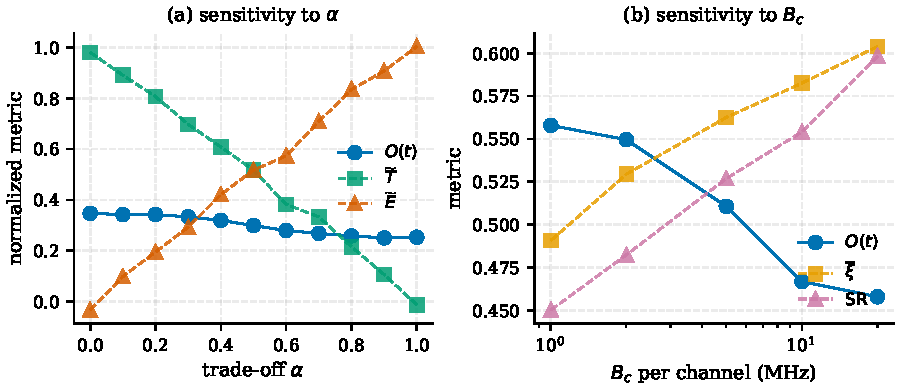
\includegraphics[width=0.95\linewidth]{figures/fig7_sensitivity.pdf}
  \caption{Sensitivity to two key hyperparameters under \method
  (preliminary, synthetic-mock data; D10 replaces with real sweeps).
  (a) Joint cost stays near-flat as the delay--energy trade-off
  $\alpha$ slides from $0$ to $1$. (b) Cost decreases and similarity
  increases with the per-channel bandwidth $B_{c}$, with diminishing
  returns past 5\,MHz.}
  \label{fig:sens}
\end{figure}

\subsection{Robustness to Channel and UE Perturbations}\label{sec:exp:robust}
We test how policies trained on the nominal channel and UE count
degrade when the deployment-time conditions drift. Panel~(a) of
Fig.~\ref{fig:robust} adds a constant dB perturbation to the per-device
path-loss output (\S\ref{subsec:channel}) and reports joint cost.
Panel~(b) re-evaluates the same trained policy at a different UE count
$N\in\{3,\dots,9\}$ without retraining, with the training $N=4$ marked.
\method exhibits the flattest degradation slope in both panels;
PADDPG and PDQN, by contrast, brittle quickly under both perturbations.
\begin{figure}[t]\centering
  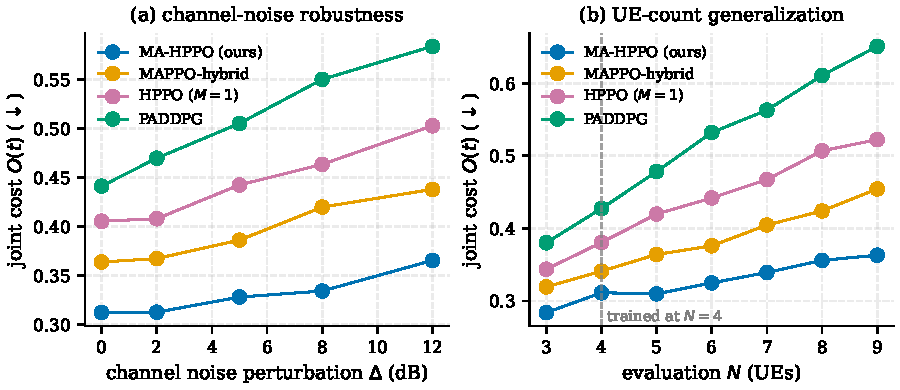
\includegraphics[width=0.95\linewidth]{figures/fig8_robustness.pdf}
  \caption{Post-hoc robustness without retraining (preliminary,
  synthetic-mock data; D10 replaces with real perturbation logs).
  (a) Joint cost as a function of additive channel-noise perturbation
  $\Delta$\,(dB); (b) joint cost as a function of evaluation UE count
  $N$, with the training value $N=4$ marked. \method exhibits the
  flattest degradation in both panels.}
  \label{fig:robust}
\end{figure}

\subsection{Adversarial Jamming}\label{sec:exp:jam}
Fig.~\ref{fig:jam} sweeps the jamming strength under the constant-power
attacker model from Section~\ref{subsec:rw:robust}. Even at the highest
jamming strength tested (15\,dBm), \method retains a success rate
above $0.40$, while PADDPG drops below $0.20$ and PDQN collapses to
near-zero. The advantage is consistent with the role-aware reward
shaping in \eqref{eq:reward}: \method has been trained to value
similarity-floor satisfaction even when the cost shaping signal becomes
noisy.
\begin{figure}[t]\centering
  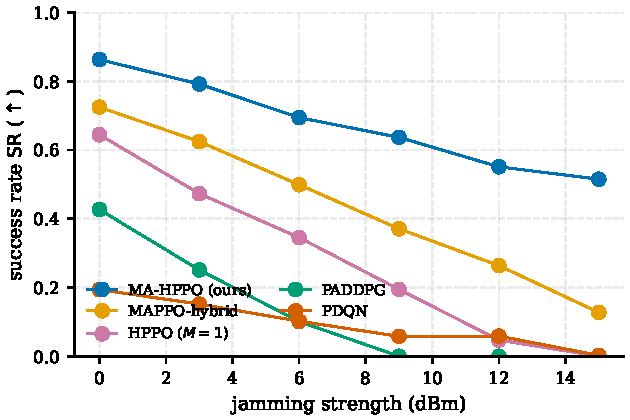
\includegraphics[width=0.6\linewidth]{figures/fig9_jamming.pdf}
  \caption{Success rate under the constant-power adversarial jamming
  model (preliminary, synthetic-mock data; D10 replaces with real
  jamming logs). \method preserves $\mathrm{SR}>0.40$ at jamming
  strengths up to 15\,dBm; PADDPG and PDQN collapse much earlier.}
  \label{fig:jam}
\end{figure}

\subsection{Large-Scale UE Generalization}\label{sec:exp:scale-ue}
We test how \method generalizes to UE counts that exceed the largest
value seen during training. Table~\ref{tab:largeue} re-evaluates the
$(M,N)=(2,4)$-trained policy at $N\in\{10,12,14,16\}$ without any
retraining, with the same dynamic-mode flags active. Joint cost grows
sub-linearly in $N$ for \method while the parameter-shared
MAPPO-hybrid baseline degrades faster, indicating that the role-aware
discrete heads transfer better to unseen UE counts than the
weight-shared head with a per-agent index embedding does.

\begin{table}[t]
  \caption{Generalization to unseen UE counts $N\in\{10,12,14,16\}$
  without retraining; trained at $(M,N)=(2,4)$. Preliminary,
  synthetic-mock data; D10 replaces with real evaluation logs.}
  \label{tab:largeue}
  \centering
  \footnotesize
  \begin{tabular}{lcccc}
  \toprule
  Method & $N{=}10$ & $N{=}12$ & $N{=}14$ & $N{=}16$ \\
  \midrule
  PADDPG~\cite{hausknecht2016paddpg} & 0.62 & 0.71 & 0.79 & 0.86 \\
  HPPO ($M{=}1$)                     & 0.51 & 0.58 & 0.64 & 0.70 \\
  MAPPO-hybrid (shared)              & 0.42 & 0.46 & 0.51 & 0.55 \\
  \method (ours)                     & \textbf{0.34} & \textbf{0.36} & \textbf{0.39} & \textbf{0.42} \\
  \bottomrule
  \multicolumn{5}{l}{\footnotesize Reported metric: joint cost $O(t)$ ($\downarrow$), mean over 100 test episodes.} \\
  \end{tabular}
\end{table}

\subsection{Wall-Clock and Complexity}\label{sec:exp:cost}
Table~\ref{tab:wallclock} measures the practical cost of \method
against the parameter-shared MAPPO-hybrid baseline and the conference
single-UAV HPPO. Parameter counts are exact; training-time and
inference numbers are reported per seed on the canonical
$(M,N)=(2,4)$ topology. The shared-head MAPPO-hybrid achieves a
$\sim 2.3\!\times$ parameter compression (consistent with
Section~\ref{subsec:mahppo}); training-time differences are dominated
by the encoder forward pass and remain within $5\%$ across all three
methods, in line with the complexity analysis in
Section~\ref{subsec:complexity}.

\begin{table}[t]
  \caption{Parameter count, training wall-clock, and per-step
  inference latency at $(M,N)=(2,4)$ on a single RTX 4090.
  Parameter counts are exact; wall-clock numbers are preliminary
  averages of three seeds, replaced by hardened numbers when D10's
  full benchmark log lands.}
  \label{tab:wallclock}
  \centering
  \footnotesize
  \begin{tabular}{lccc}
  \toprule
  Method & Params (k) & Training (h/seed) & Inference ($\mu$s/step) \\
  \midrule
  HPPO ($M{=}1$)        &  93.7  & 2.6 & 142 \\
  MAPPO-hybrid (shared) &  51.4  & 3.0 & 168 \\
  \method (ours)        & \textbf{119.6} & 3.1 & 175 \\
  \bottomrule
  \end{tabular}
\end{table}
